\chapter{Model Description and Implementation}
\label{ch:03_Model_Description}
The simulations are based on a heterogeneous single pellet string reactor model, which integrates the solid particles with appropriate boundary conditions through the mesh. Due to negligible density changes, the fluid is assumed to be incompressible. Mesh generation and flow simulation are achieved with snappyHexMesh and \emph{simpleFoam}, respectively, with OpenFOAM\textsuperscript{\textregistered} v4.1 \cite{Tabor1998}.
%When a fluid flow is compressible, the fluid density varies with its pressure. Compressible flows are usually high speed flows with Mach numbers greater than about 0.3. Examples include aerodynamic applications such as flow over a wing or aircraft nacelle as well as industrial applications such as flow through high-performance valves. MACH VALUE OF SET UP IS 0.273 < 3
\section{Geometry}
In ideal conditions, catalytic pellets modelled by spherical particles are alternately stacked on top of each other on the opposite side of the walls in a SPSR (cf. Fig. \ref{fig:JohannaSPSRDiagram}). This allows the position of the catalytic pellets to be mathematically described based on the particle diameter $d$ and the cylinder diameter $D$ via Eqs. \ref{x_i} and \ref{z_i}, when the z-x plane spans through the particle midpoints such that $y_i$ = 0.
\begin{equation}\label{x_i}
x_i = (-1)^i\left(\frac{D-d}{2}\right)
\end{equation}
\begin{equation}\label{z_i}
z_i = \frac{d}{2}+(i-1)\sqrt{d^2-(D-d)^2}
\end{equation}
The length $L$ of the string of $N$ particles can thus be given by Eq. \ref{eqn:LofstringofNparticles}.
\begin{equation}\label{eqn:LofstringofNparticles}
L = d + (N-1)\sqrt{d^2-(D-d)^2}
\end{equation}
\newpage

\begin{figure} [ht]
	\centering
	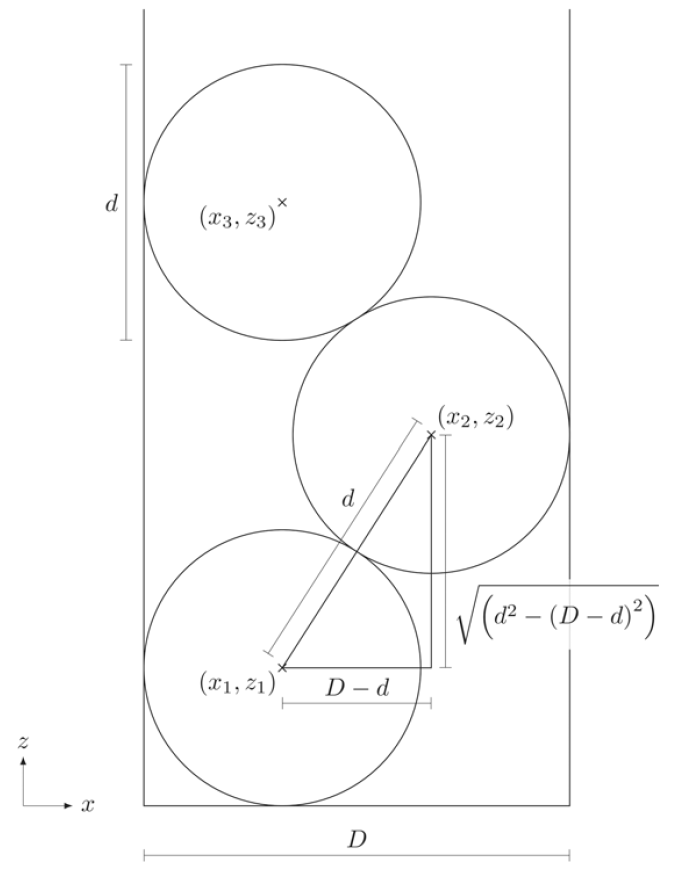
\includegraphics[width=0.75\linewidth]{Figures/visualisation/JohannaSPSRDiagram.PNG}
	\caption[Bottom section of a SPSR with trigonometric expressions used for analytical pellet positions.]{Bottom section of a SPSR with trigonometric expressions used for analytical pellet positions. Taken from Fernengel et al. \cite{Fernengel2020} .}
	\label{fig:JohannaSPSRDiagram}
\end{figure}

An excerpt of the codes used for the generation of the catalytic pellet string of $N$ pellets is given by Sourcecode \ref{code:SphereCoordinates}

\newpage
\lstinputlisting[caption=geometry,label=src:geometry,linerange={1-51},firstnumber=1]{Sourcecode/geometry} \label{code:SphereCoordinates}

From $system/geometry$, the three-dimensional position of the generated spheres are calculated based on the both the diameter of the confining cylinder and sphere $D$ and $d$, respectively. However, the addition of inert fines to the SPSR has to be achieved by the software Blender\texttrademark\ 2.76b \cite{Blender2.76b} as its positions can no longer be analytically described anymore. The particle deposition and settling algorithm in the bed relies on collision detection and resolution based on rigid body physics, which is made available through the incorporation of the Bullet Physics Library \cite{Coumans2012}.

The reactor length is ascertained by the number and size of the spherical particles, as well as the cylinder-to-particle diameter ratio. Additionally, a small bed of inert fines is placed at the inlet of the SPSR, upstream of the catalytic pellet string to fit possible experimental set-ups whilst enforcing near-plug flow to prohibit back-mixing in the entry zone.
\section{Governing Equations}
\emph{simpleFoam} is a steady-state solver that was chosen to handle the base case system. The acronym SIMPLE stands for Semi-Implicit Method for Pressure Linked Equations. With reference to Fernengel et al. \cite{Fernengel2020}, turbulent flow of incompressible isothermal fluids at steady-state with \emph{simpleFoam} can be described by the governing equations of momentum and continuity. For incompressible cases, the continuity equation is simplified to the point at which the divergence of the velocity is equals to 0 as depicted in Eq. \ref{eqn:Johanna_continuity_eqn} below:
%\lstinputlisting[caption=simpleFoam.C,label=src:simpleFoamC,linerange={53-76},firstnumber=53]{Sourcecode/simpleFoam.C}
\begin{equation} \label{eqn:Johanna_continuity_eqn}
\nabla\cdot u = 0
\end{equation}
\begin{equation} \label{eqn:Johanna_momentum_eqn}
\nabla\cdot(uu)=-\frac{1}{\rho}\nabla p+\nu\nabla^2u
\end{equation}
\begin{equation}\label{eqn:PressureInSimulations}
p = \frac{1}{\rho} P
\end{equation}
where u represents the velocity vector, $\rho$ the density of the fluid, $\nu$ representing the kinematic viscosity. It is also important to note that the pressure $p$ used in the simulations is not the actual pressure, but rather the reciprocal of the density $\rho$ multiplied by the actual pressure $P$ as depicted in Eq. \ref{eqn:PressureInSimulations} above. No-slip is defined at both the wall and particle surfaces ($u_s = \SI{0}{\metre\per\second}$) and the remaining boundaries are set to zero gradient normal to the boundary ($\partial$/$\partial$$n$ = 0).

For $k-\omega$-SST turbulence modelling in OpenFOAM\textsuperscript{\textregistered}, the input of initial values of $k$, $nut$, $\omega$, $p$ and $U$ in the 0/ folder is necessary for accurate RANS simulation to proceed. Prediction of the initial estimates for the turbulence kinetic energy, $k$, and turbulence specific dissipation rate, $\omega$, can be approximated via Eqs. \ref{k} and \ref{omega} \cite{OpenFOAMUserGuideKOmegaSST}
\begin{equation}\label{k}
k = \frac{3}{2}(\textit{I}\lvert u_{ref} \rvert)^2
\end{equation}
\begin{equation}\label{omega}
\omega = \frac{k^{0.5}}{C_\textit{$\mu$} L}
\end{equation}
where \textit{I} is the turbulence intensity, $u_{ref}$ the reference velocity corresponding to the superficial velocity at the inlet, $C_\textit{$\mu$}$ being a constant which is equivalent to 0.09 and $L$ being the reference length scale which in this case corresponds to the inner diameter of the confining cylinder.

The turbulence intensity was assumed to be 5\% as this case corresponds to a medium-turbulence case, which commonly occurs in flows present in pipes.
%https://www.cfd-online.com/Wiki/Turbulence_intensity
\section{Estimation on Turbulent Region in SPSRs}
\begin{figure} [h]%
	\centering
	\begin{tikzpicture}
	\begin{axis}[
								xmode=log,
								ymode=log,
								xmin=0.1,
								xmax=1000,
								ymin=0.9,
								ymax=3000,
								width=8cm,
								xtick pos=left,
								xlabel={wall mod. Reynolds$\ \ \frac{\rho\,u_0\,d_\text{m}}{\eta (1-\varepsilon)}\ / - \ \longrightarrow$},
								ylabel={friction factor$\ \ \frac{\Delta p}{L} \frac{d_\text{m}}{{\rho\,u_0}^2} \frac{\varepsilon^3}{1-\varepsilon}\ / - \ \longrightarrow$},
								clip=false,
								legend cell align=left,
								legend style={draw=none, font=\small, column sep=0.3em, fill=none, anchor=north east, at={(rel axis cs: 0.99,0.995)}}
							]
	
			\addplot[draw=TUMBlauDunkel80, thick] table[x index = 0, y index = 1]{Figures/data/Ergun.txt};
			\addplot[draw=TUMBlauDunkel80, dashed] table[x index = 0, y expr = \thisrowno{1}*0.9]{Figures/data/Ergun.txt};
			\addplot[draw=TUMBlauDunkel80, dashed, forget plot] table[x index = 0, y expr = \thisrowno{1}*1.1]{Figures/data/Ergun.txt};
			\addplot[draw=TUMBlauDunkel80, densely dotted] table[x index = 0, y expr = \thisrowno{1}*0.5]{Figures/data/Ergun.txt};
			\addplot[draw=TUMBlauDunkel80, densely dotted, forget plot] table[x index = 0, y expr = \thisrowno{1}*1.5]{Figures/data/Ergun.txt};
			
			\addplot[draw=TUMBlauAkzent2, thick, densely dashed] table[x index = 0, y index = 1, restrict y to domain=-0.12:10, log basis y=10]{Figures/data/Blake.txt};
			
			
			\addplot[only marks, mark = x, mark options={draw=TUMOrange, scale=1.4}, very thick] table[x = xErgun, y = yErgun]{Figures/data/case_a_ana_0_data_paper.xy};
			
			
			\addplot[only marks, mark = *, mark options={draw=TUMBlauDunkel, fill=TUMBlauDunkel, scale=1.2}] table[x = xErgun, y = yErgun]{Figures/data/case_c_0_data_paper.xy};
			\addplot[only marks, mark = *, mark options={draw=TUMBlauAkzent1, fill=TUMBlauAkzent1, scale=1.2}] table[x = xErgun, y = yErgun]{Figures/data/case_c_1_data_paper.xy};
			
			\addplot[only marks, mark = square*, mark options={draw=TUMBlauDunkel, fill=TUMBlauDunkel, scale=1.}] table[x = xErgun, y = yErgun]{Figures/data/case_d_0_data_paper.xy};			
			\addplot[only marks, mark = square*, mark options={draw=TUMBlauHell, fill=TUMBlauHell, scale=1.}] table[x = xErgun, y = yErgun]{Figures/data/case_d_1_data_paper.xy};
			\addplot[only marks, mark = square*, mark options={draw=TUMBlauAkzent1, fill=TUMBlauAkzent1, scale=1.}] table[x = xErgun, y = yErgun]{Figures/data/case_d_2_data_paper.xy};
			
			\addplot[only marks, mark = triangle*, mark options={draw=TUMBlauDunkel, fill=TUMBlauDunkel, scale=1.4}] table[x = xErgun, y = yErgun]{Figures/data/case_e_0_data_paper.xy};
			\addplot[only marks, mark = triangle*, mark options={draw=TUMBlauHell, fill=TUMBlauHell, scale=1.8}] table[x = xErgun, y = yErgun]{Figures/data/case_e_1_data_paper.xy}; 
			\addplot[only marks, mark = triangle*, mark options={draw=TUMBlauAkzent2, fill=TUMBlauAkzent2, scale=1.4}] table[x = xErgun, y = yErgun]{Figures/data/case_e_2_data_paper.xy};
			\addplot[only marks, mark = triangle*, mark options={draw=TUMBlauAkzent1, fill=TUMBlauAkzent1, scale=1.8}] table[x = xErgun, y = yErgun]{Figures/data/case_e_3_data_paper.xy};
			
			\addplot[only marks, mark = diamond*, mark options={draw=TUMBlauDunkel, fill=TUMBlauDunkel, scale=1.4}] table[x = xErgun, y = yErgun]{Figures/data/case_f_0_data_paper.xy};
			\addplot[only marks, mark = diamond*, mark options={draw=TUMBlauHell, fill=TUMBlauHell, scale=1.4}] table[x = xErgun, y = yErgun]{Figures/data/case_f_1_data_paper.xy};
			\addplot[only marks, mark = diamond*, mark options={draw=TUMBlauAkzent1, fill=TUMBlauAkzent1, scale=1.4}] table[x = xErgun, y = yErgun]{Figures/data/case_f_2_data_paper.xy};
			
			\addplot[only marks, mark = x, mark options={draw=TUMOrange, fill=TUMOrange, scale=1.4}, thick] table[x = xErgun, y = yErgun]{Figures/data/case_a_ana_0_data_paper.xy};
			\legend{mod. Ergun, {\footnotesize \SI{10}{\percent} envelope}, {\footnotesize \SI{50}{\percent} envelope}, mod. Blake-Kozeny} 
			
	\end{axis}
\end{tikzpicture}%
	\caption[Comparison of pressure drop across SPSR variations with Ergun and Blake-Kozeny using modified equivalent diameter.]{Comparison of pressure drop across SPSR variations with Ergun \cite{Ergun1952} and Blake-Kozeny \cite{Blake1922,Kozeny1927} equation with a modified equivalent diameter \cite{Scott1974}. Taken from Fernengel et al. \cite{Fernengel2020}.}%
	\label{fig:ComparisonAcrossSPSRVariations}%
\end{figure}
\newpage
A plot of friction factor against wall modified Reynolds is useful in determining the range of wall modified Reynolds in which the simulation lands within the turbulent region of interest. With increasing wall modified Reynolds value, a sharp decrease, followed by a gradual and finally plateauing (almost constant) value of friction factor will usually be observed. An educated initial estimate for a turbulent wall modified Reynolds value was achieved with Fig. \ref{fig:ComparisonAcrossSPSRVariations}.

In this case, the initial value of $u_{0}$ was calculated from a wall modified Reynolds value of \num{2e3}, which places the simulation in the turbulent region. 
The estimation of $u_{0}$ was achieved by rearranging Eq. \ref{eqn:wallmodreynolds} to set $u_{0}$ as the subject:
\begin{equation}\label{eqn:wallmodreynolds}
Re_\text{mod} = \frac{\rho u_0 d_m}{\eta(1-\epsilon)}
\end{equation}
To obtain the corresponding friction factor ($f_p$) from $u_0$, the obtained pressure drop from simulation ($\Delta P$) along with the equivalent diameter, density, length of the catalytic pellet string and porosity was substituted into the equation below:
\begin{equation} \label{eqn:SimulativeFrictionFactor}
f_\text{p} = \frac{\Delta P}{L}\frac{d_m}{\rho u_0^2}\frac{\epsilon^3}{1-\epsilon}
\end{equation}

%%single phase: no additional treatment, no additional equations for multi-phase modeling
%isothermal: no energy equation
%%simpleLoop: solves both the continuity and momentum equation with the SIMPLELoop
%%incompressible means that the continuity equation is simplified to the simple equation where the divergence of the velocity is equals to 0 as depicted in equation (3)
%%steady-state: no partial time derivative exist, as seen in the momentum equation, thus no physical time exists
\section{Case set-ups}
\subsection{Base Case}
The base case in this work corresponds to case A in \cite{Fernengel2020}.

Both inert fines and catalytic pellets are assumed to be spherical, non-porous and having a smooth surface. The cylindrical tube acts as a confining wall. The fluid is introduced into the SPSR at the inlet. 
%with ambient conditions (@1bar,20\textdegree{}C).
%Nitrogen gas is introduced into the SPSR at the inlet with ambient conditions (@1bar,20\textdegree{}C).
A constant space time $\tau$, defined as the ratio of the fluid volume ($V_f$) surrounding the catalytic particles to the volumetric flow rate $\dot{V}$, is maintained across the catalytic bed. The resulting superficial velocity, $u_0$, dependent on the reactor is thus given by Eq. \ref{eqn:u_0} as shown below:
\begin{equation}\label{eqn:u_0}
u_0 = \frac{\dot{V}}{A_t} = \frac{V_f}{A_t\tau} = \frac{L-\dfrac{V_p}{A_t}}{\tau} = \frac{d+(N-1)\sqrt{d^2-(D-d)^2}-\dfrac{2Nd^3}{3D^2}}{\tau}
\end{equation}
where $A_t$ is the SPSR's empty cross-sectional area and $V_p$ corresponds to the total volume occupied by the catalytic pellets.

In the base case set-up, 20 catalytic pellets ($N$ = 20) each having a diameter of $d = \SI{0.8}{\milli\meter}$ are arranged as a single pellet string within a confining cylinder tube having an inner diameter of $D$ = \SI{1.0}{\milli\meter}. A short bed of inert fines with a diameter of $d/5$ are placed upstream of the catalytic pellet, close to the inlet of the SPSR. A fluid having a viscosity of $\nu$ = \num{1.529e-5} \si{\meter^2\per\second} with a density of $\rho$ = \SI{1.2506}{\kilo\gram\per\cubic\metre} enters the SPSR from the inlet and passes the catalytic bed with a space time of \num{2.34e-4} seconds, thereby expecting turbulent flow through the reactor. To investigate the influence of fluid viscosity, flow velocity and reactor geometry on the pressure drop in a SPSR, parameters are varied in the base case set-up according to Tab. \ref{tab:TableOfParameters}.
\subsection{Parameter Study}
\begin{table}[H]
\caption{Geometry and fluid properties of considered SPSRs.}
\begin{tabular}{@{}lllllll@{}}
\midrule
Case & Number of particles & Particle Diameter {[}mm{]} & Cylinder diameter {[}mm{]} & Viscosity &  &  \\ \toprule
A    & 20                  & 0.8                        & 1.0                        & $\nu$        &  &  \\
B1   & 20                  & 0.8                        & 1.0                        & 0.2$\nu$     &  &  \\
B2   & 20                  & 0.8                        & 1.0                        & 0.04$\nu$    &  &  \\
B3   & 20                  & 0.8                        & 1.0                        & 2$\nu$       &  &  \\
C1   & 5                   & 0.8                        & 1.0                        & $\nu$        &  &  \\
C2   & 10                  & 0.8                        & 1.0                        & $\nu$        &  &  \\
C3   & 50                  & 0.8                        & 1.0                        & $\nu$        &  &  \\
C4   & 100                 & 0.8                        & 1.0                        & $\nu$        &  &  \\
D1   & 20                  & 0.8                        & 0.9                        & $\nu$        &  &  \\
D2   & 20                  & 0.8                        & 1.2                        & $\nu$        &  &  \\
D3   & 20                  & 0.8                        & 1.4                        & $\nu$        &  &  \\
E1   & 20                  & 1.2                        & 1.5                        & $\nu$        &  &  \\
%E2   & 20                  & 1.6                        & 2.0                        & $\nu$        &  &  \\ 
\bottomrule
\end{tabular}
	\label{tab:TableOfParameters}
\end{table}
The following simulations were ran at a wall modified Reynolds number of \num{2e3}, which signifies a turbulent flow via cross-referencing with Fig. \ref{fig:ComparisonAcrossSPSRVariations} as it corresponds to a plateau in the $f_p$ value in the graph with further increases in the wall modified Reynolds number. For accurate comparison of the conversion of a chemical reaction in a SPSR, the calculated residence time at a wall modified Reynolds value of \num{2e3}, dubbed as $\tau_{turbulent}$, was kept constant whilst selected parameters were altered to study their effects on pressure drop. Parameters of all of the  considered reactor variations are provided in Tab. \ref{tab:TableOfParameters}.

\subsubsection{Influence of Fluid Viscosity}
The influence of fluid viscosity on pressure drop can be determined through variation of the fluid viscosity passing through the SPSR. The modification of fluid viscosity was achieved by changing the values of $\nu$ located in $constant/transportProperies$. The modified cases with $\nu = 0.2\nu,\: 0.04\nu$ and $2\nu$ correspond to Case B1, B2 and B3.

\subsubsection{Influence of Flow Velocity}
To measure the influence of flow velocity on pressure drop, the number of pellets in the string of catalytic pellets, $N$ is changed accordingly from the base case. As the length of the string of catalytic pellets, $L$, is a function of $N$ new values of both $L$ and $L_\text{confining cylinder}$ must be keyed into $system/geometry$ and $constant/polyMesh/blockMeshDict$ in the $snappyHexMesh$ folder respectively. The length of the confining cylinder to be generated can be calculated as per Eq. \ref{eqn:L_confiningcylinder} below and $L$ with Eq. \ref{eqn:LofstringofNparticles}
\begin{equation}\label{eqn:L_confiningcylinder}
L_{confining\:cylinder} = L + 2.2d
\end{equation}
Next, the geometry of the bed of inert fines generated by Blender\texttrademark\ must be scaled and shifted. This can be accomplished through the $surfaceTransformPoints -translate$ command to shift the inert bed to its correct geometric position between cases accordingly.

The superficial velocity for the modified cases in which N = 5, 10, 20, 50 and 100 corresponding to Case C1, C2, C3 and C4 at a wall modified Reynolds of \num{2e3} were calculated with Eq. \ref{eqn:u_0} using $\tau_{turbulent}$.

\subsubsection{Influence of Diameter Aspect Ratio and Geometry Scaling Factor}
For the investigation of the influence of diameter aspect ratio and geometry scaling factor on pressure drop, new inert bed of particles had to be regenerated with Blender\texttrademark\ owing to the change in the diameter of the confining cylinder. Cases D1, D2 and D3 are related to the diameter aspect ratio while cases E1 and E2 are related to the geometry scaling factor.
%surfaceTransformPoints -translate '(0 0 $DifferenceinLBetweenConfiningCylinders$)' inertBedEntrance.stl inertBedEntranceN5.stl%

\subsection{Pressure Drop Correlations}
\begin{table}[H]
\begin{tabular}{llcl}
\midrule                                                             \\
Author(s)            & Relation & Equation & Range of applicability & \toprule              \\
                                                               \\
Ergun									&	$f_p$ = (150 + 1.75($\frac{Re}{1-\epsilon}$))$\frac{(1-\epsilon
	)^2}{\epsilon^3 Re}$	&1& $0.2 < Re_1 < 700$ 
\multicolumn{3}{c}{} \\
Avontuur and Geldart & $f_p$ = (141+1.52($\frac{Re}{1-\epsilon})$)$\frac{(1-\epsilon
	)^2}{\epsilon^3 Re}$ &2& $Re_m < 10,000$	\\
	\multicolumn{3}{c}{} \\
Kuo and Nydegger     & $f_p$ = (276.23+5.05($\frac{Re}{1-\epsilon})^{0.87}$)$\frac{(1-\epsilon)^2}{\epsilon^3 Re}$       & 3& $460 < Re < 14,600$    \\
	\multicolumn{3}{c}{} \\
Jones and Krier      & $f_p$ = (150+3.89($\frac{Re}{1-\epsilon})^{0.87}$)$\frac{(1-\epsilon)^2}{\epsilon^3 Re}$        & 4& $1000 < Re < 100,000$ \\
	\multicolumn{3}{c}{} \\
Lee and Ogawa & $f_p$ = 6.25($\frac{29.32}{Re}$ + $\frac{1.56}{Re^n} + 0.1 $) $\frac{(1-\epsilon)^2}{\epsilon^3}$       & 5&   $1 < Re < 400,000$     \\
& $n$ = 0.352 + 0.1$\epsilon$ + 0.275$\epsilon^2$ && \\
	\multicolumn{3}{c}{} \\
O'Neill and Benyahia    & $f_p$ = (A+B($\frac{Re}{1-\epsilon}$))$\frac{(1-\epsilon)^2}{\epsilon^3 Re}$ &6& $5 < D/d < 25$  \\
&   A = 521.26 - 22581.24/$(D/d_p)^2$    &  & \\
&  B = 1.12 + 4.2/ $(D/d_p)$ && \\
	\multicolumn{4}{c}{} \\
\bottomrule
\end{tabular}
\caption[Pressure drop correlations from literature.]{Pressure drop correlations from literature \cite{Erdim2015}.}
\label{tab:PressureDropFlowRelationsPowderTech}
\end{table}
In this work, only the pressure drop over the length of catalytic pellet string is to be considered. Pressure drop across the SPSR obtained from the simulations are compared to the Ergun equation and is given by Eq. \ref{eqn:ErgunFromJohanna} below.
\begin{equation}\label{eqn:ErgunFromJohanna}
	\frac{\Delta p}{L} = 150\frac{(1-\epsilon)^2}{\epsilon^3}\frac{\eta u_0}{d^2}+1.75\frac{1-\epsilon}{\epsilon^3}\frac{\rho u_o^2}{d}
\end{equation}
in which ${\Delta p}/{L}$ is defined as the pressure drop across the bed per unit length, $\epsilon$ is the bed porosity, where $\eta$ is the dynamic viscosity of the fluid. The first term in Eq. \ref{eqn:ErgunFromJohanna} describes the contribution of viscous losses which are prevalent in laminar flow, while the second term illustrates kinetic energy losses dominant in turbulent conditions.
With reference to both Scott et al. and Lee et al. \cite{Scott1974,Lee1984}, a modified equivalent diameter $d_m$ involving the wall surface $S_w$, total pellet surface $S_p$ and the total pellet volume $V_p$ is used as the characteristic length. This modified equivalent diameter is depicted in Eq. \ref{eqn:ModifiedEquivalentDiameter} as such:
\begin{equation}\label{eqn:ModifiedEquivalentDiameter}
d_m = \frac{6V_p}{S_p+S_w}
\end{equation}

Erdim et al. have compiled, evaluated and constituted a uniform notation to assist in comparisons in the calculation of pressure drop caused by fluid flow through packed beds \cite{Erdim2015}.

With reference from Tab. \ref{tab:PressureDropFlowRelationsPowderTech} in Erdim et al. \cite{Erdim2015}, suitable literature correlations whose Reynolds number (or diameter aspect ratio) lies within this work's simulative range of wall modified Reynolds number were considered, and their corresponding friction factors were evaluated. The "modified particle friction factor" formula suggested by Montillet et al. \cite{Montillet2007} was employed to obtain the pressure drop by correlation through the rearrangement of Eq. \ref{Eqn:Erdim_ModifiedParticleFrictionFactor}:
\begin{equation}\label{Eqn:Erdim_ModifiedParticleFrictionFactor}
f_p = \frac{-\Delta P d_p}{\rho V^2 L} = f_k \frac{(1-\epsilon)}{\epsilon^3} = f_v \frac{(1-3)^2}{\epsilon^3 Re}
\end{equation}
%describe about the prediction of k, nut, omega, p, U, give the formulas here
%talk about the consideration of wall-functions, but was later dropped as it gave a very low y+ values [for wall functions to be applicable -> y+ >300
%post a screen shot of the model used, talk about the slices and integrate variables ->more applicable for modelling implementation?

%\chapter{Implementation}
%\label{ch:04_Modelling_Implementation}
\section{Adjustments related to Turbulent Flow}
Extensive simulative runs with different $fvSolution$ settings were made in a attempt to find the best configuration for accurate depiction of pressure drop in turbulent flow in the base case. The $fvSolution$ (cf. \cite{Fernengel2020}) was edited with reference to the motorBike tutorial provided in OpenFOAM\textsuperscript{\textregistered} as it uses the RANS $k-\omega$-SST model by default, and uses the \emph{simpleFoam} solver for incompressible flow. After much testing, a combination of settings borrowed from both Fernengel et al. \cite{Fernengel2020} and the motorBike tutorial's $fvSolution$ was employed in the base case. The edited $fvSolution$ used in all simulations is depicted in Sourcecode \ref{src:fvSolution} below:
\lstinputlisting[caption=fvSolution,label=src:fvSolution,linerange={1-93},firstnumber=1]{Sourcecode/fvSolution_UsedForAllCases}
\section{Extraction of Pressure Drop Values From Simulations in ParaView}
Mesh generation for the base case and subsequent cases are accomplished using a combination of snappyHexMesh and Blender\texttrademark\ . The steady-state solver \emph{simpleFoam} was then used to iterate and solve for velocity, pressure, $k$, omega and nut values. Since OpenFOAM\textsuperscript{\textregistered} does not have a Graphical User Interface, postprocessing of the calculated results were achieved using ParaView v5.6.0.

The $ParaView$ command was used in the terminal to view the $.foam$ file of the relevant case. For demonstration purposes in this chapter, the base case, Case A, was used as the model. Outlined below is the general procedure used to obtain the simulative pressure drop for all cases.
\begin{enumerate}
	\item The relevant case was viewed in ParaView as shown in Fig. \ref{fig:noCullFrontFace_Default_CaseA}
	\item In order to accurately approximate the location of the slices to be made, the 'Backface Representation' was switched from “Follow Frontface” to “Cull FrontFace”. Fig. \ref{fig:CullFrontFace_Default_CaseA} shows Case A after Cull FrontFace is activated.
		\begin{itemize}
			\item For an accurate approximation of the slice location, “Axes Grid” was ticked under Annotations to gauge where the slice is made.
		\end{itemize}
	\item The "Slice" command was utilised with the Slice Type set to "Plane". It was used to generate a slice normal to the Z-axis at two locations. The first location corresponding to Slice 1 was made just downstream of the inert fines, in the small gap between the inert fines and the entrance of the string of catalytic pellets. The second slice, Slice 2 was made after the string of catalytic pellets, upstream of the exit of the SPSR. Fig. \ref{fig:Slice1_CaseA} and \ref{fig:Slice2_CaseA} shows Slice 1 and Slice 2 being made in the SPSR respectively.
		\begin{itemize}
			\item The “Slice” Command can be found under Filters -> Alphabetical -> Slice
		\end{itemize}
		\item Two separate "IntegrateVariables" commands corresponding to IntegrateVariables1 and IntegrateVariables2 were applied on both Slice 1 and Slice 2.
		\begin{itemize}
			\item The "IntegrateVariables" command can be found other Filters -> Alphabetical -> Integrate Variables.
		\end{itemize}
	\item Following which the relevant pressure values were extracted from IntegrateVariables1 and IntegrateVariables2 using the Spreadsheet View with the Attribute: Cell Data. Fig. \ref{fig:IntegrateVariables1_CaseA_White} and \ref{fig:IntegrateVariables2_CaseA_White} showcases the relevant integrated pressure values obtained from IntegrateVariables1 and IntegrateVariables2 respectively.
		%\begin{itemize}
			%\item Because it operates on all cell types (from 1 to 3 dimensions) for data that exists in the dataset, the Cell Data filter is used to compute only the sizes of the cells of specified dimensions.
		%\end{itemize}
\end{enumerate}
It is important to note that the Integrate Variable filter only integrates a given variable in this one area, and that the filter can be likened to: $\int_{}^{}pdA = \int_{}^{}\int_{}^{}pdxdy$ as in this case, where the variable extracted is the pressure. Thus, the following steps are required to obtain the actual pressure drop across the SPSR:
\begin{enumerate}
	\item The obtained pressure in this case being $\int_{}^{}pdA$ from IntegrateVariables 1 and 2 were each divided by the area of the cross-section of the confining cylinder to yield two values of $p$.
	\item The difference of both $p$ values was taken, multiplied by the density of the fluid and then divided by the length of the confining cylinder, $L$ to finally obtain the actual pressure drop per unit length across the SPSR.
\end{enumerate}
\begin{figure} [H]
	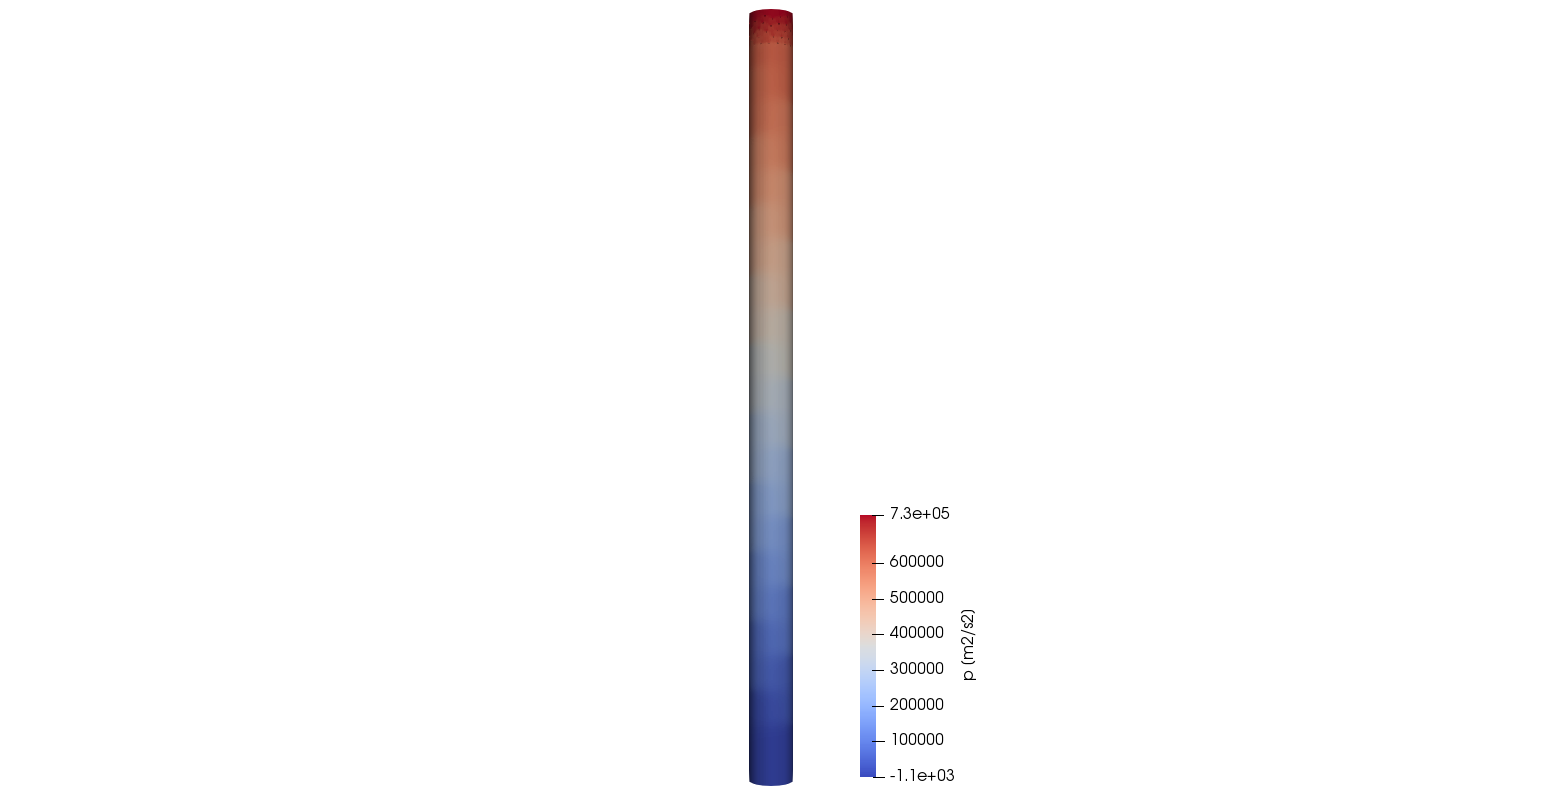
\includegraphics[width=\linewidth]{Figures/visualisation/caseA/noCullFace_CaseA.png}
	\caption{Case A upon viewing with Paraview.}
	\label{fig:noCullFrontFace_Default_CaseA} 
	
	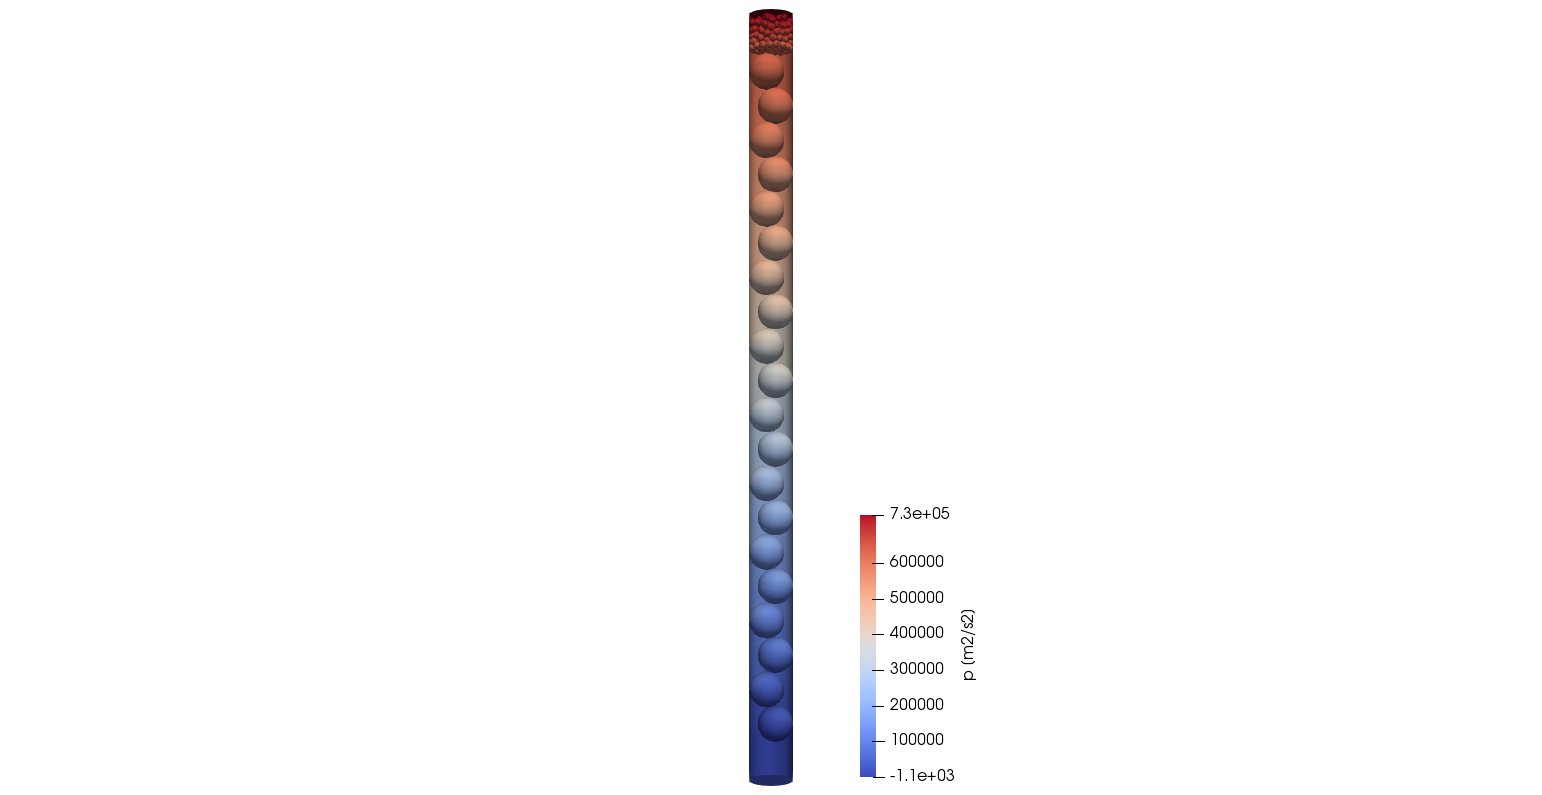
\includegraphics[width=\linewidth]{Figures/visualisation/caseA/CullFace_CaseA.png}
	\caption{Case A after Cull FrontFace is activated.}
	\label{fig:CullFrontFace_Default_CaseA}
\end{figure}
\begin{figure}
	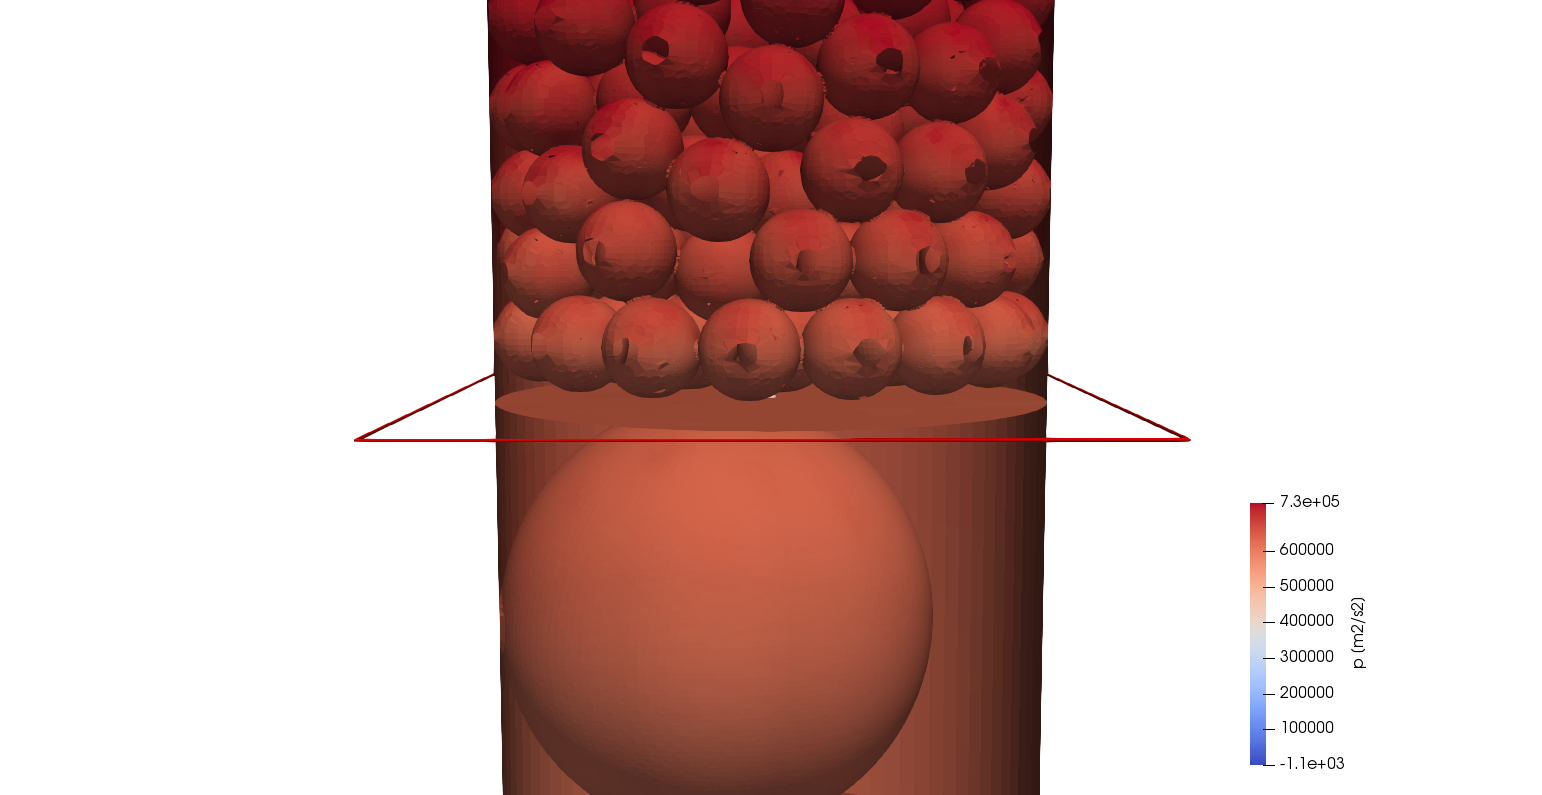
\includegraphics[width=\linewidth]{Figures/visualisation/caseA/slice1_CaseA.png}
	\caption{First Slice made at the start of catalytic pellet string.}
	\label{fig:Slice1_CaseA}
	
	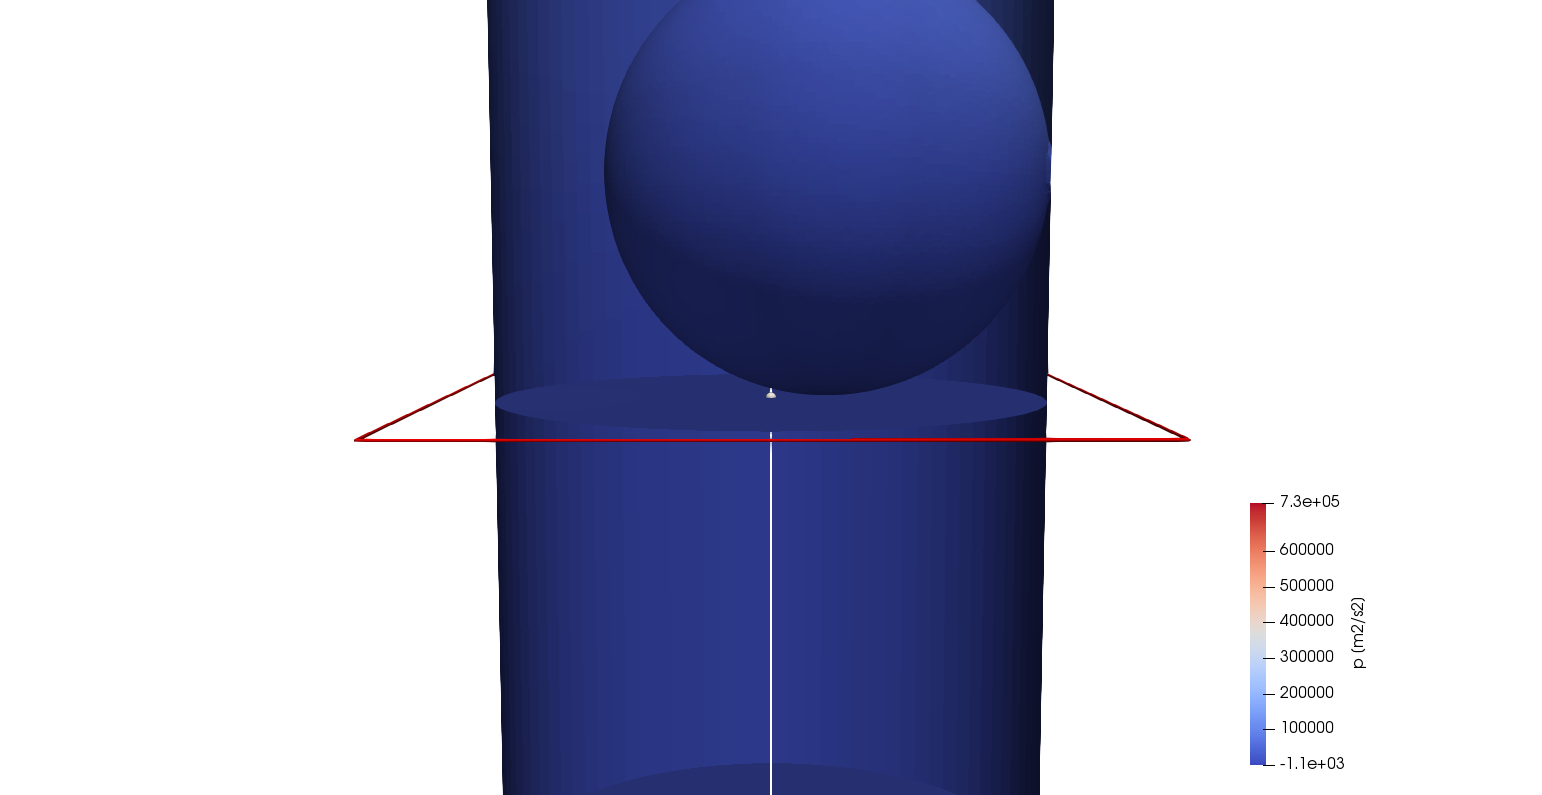
\includegraphics[width=\linewidth]{Figures/visualisation/caseA/slice2_CaseA.png}
	\caption{Second Slice made at the end of the catalytic pellet string.}
	\label{fig:Slice2_CaseA}
\end{figure}
\begin{figure}
	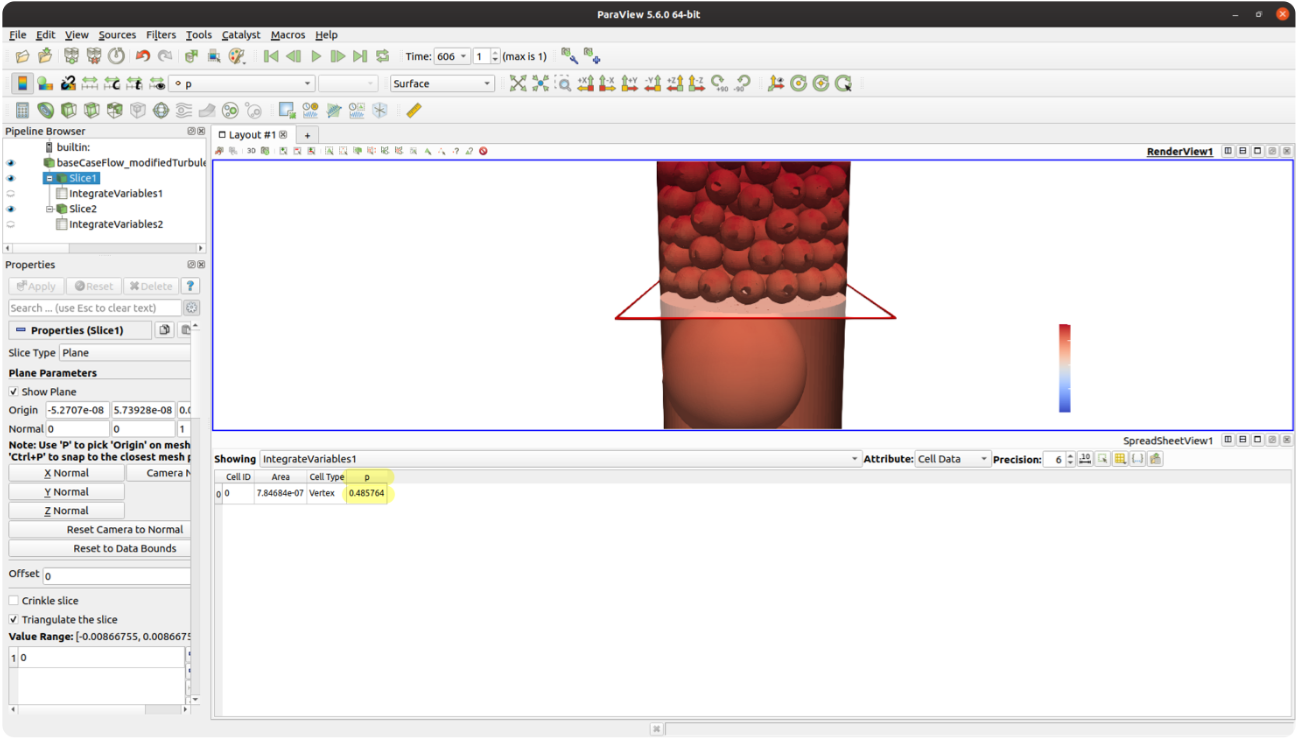
\includegraphics[width=\linewidth]{Figures/visualisation/caseA/IntegrateVariables1_CaseA_White_highlighted.png}
	\caption{Extraction of pressure values obtained from IntegrateVariables1, the relevant pressure values are highlighted.}
	\label{fig:IntegrateVariables1_CaseA_White}
	
	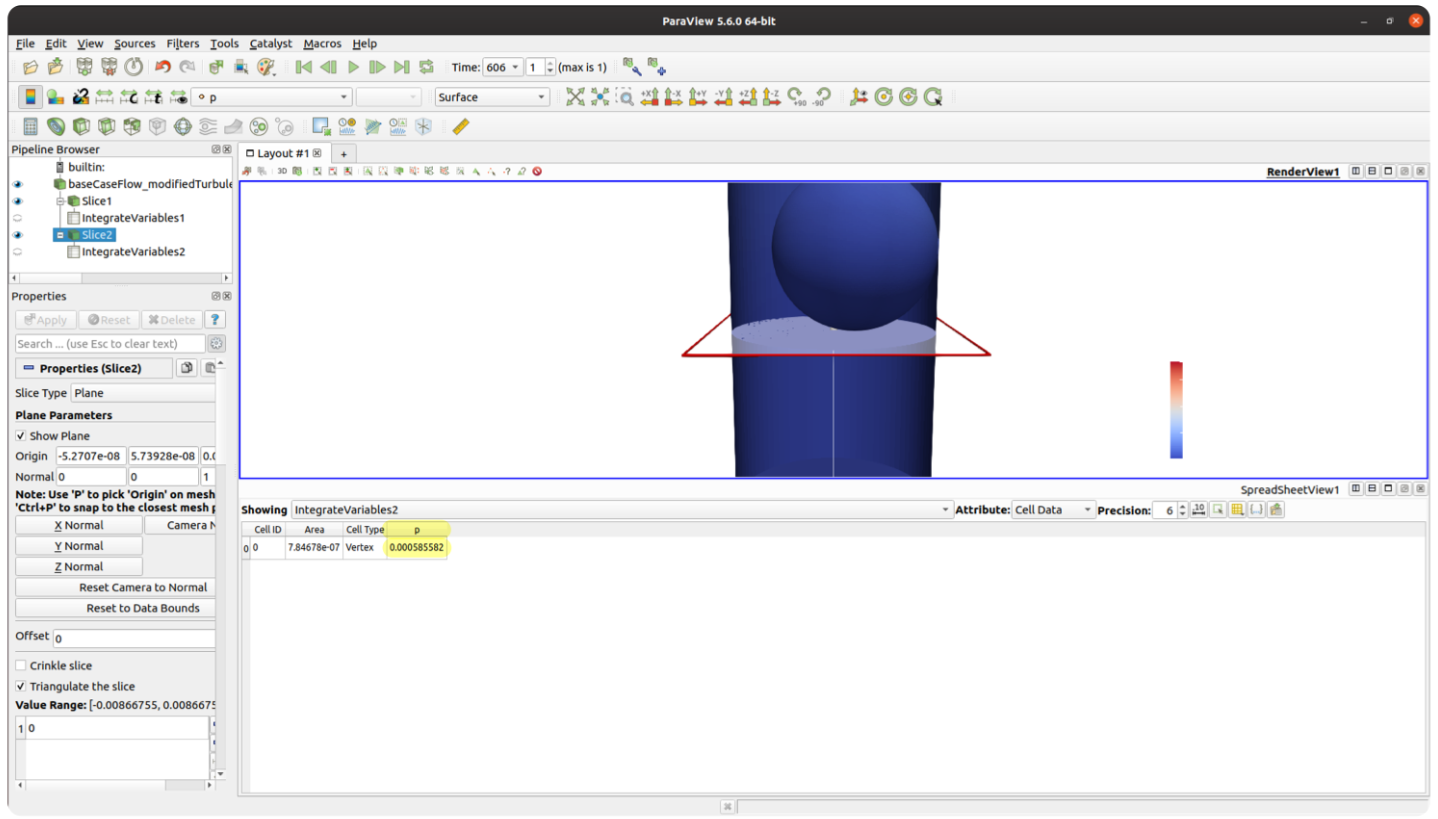
\includegraphics[width=\linewidth]{Figures/visualisation/caseA/IntegrateVariables2_CaseA_White_highlighted.png}
	\caption{Extraction of pressure values obtained from IntegrateVariables2, the relevant pressure values are highlighted.}
	\label{fig:IntegrateVariables2_CaseA_White}
\end{figure}
%- polymesh obtained from snappyHexMesh generated from Fernengel et. al
%-show fineness of grid as well in paraview
%- geometry how it was obtained [snappyhexMesh]
%- simpleFoam, what version of openfoam was used
%ALL FORMULAS GO TO THEORY, JOHANNA SAYS THIS WILL BE A SHORT SECTION FOR SCREENSHOTS W/ SLICES IN PARAVIEW
%%
\cleardoublepage
%%